\documentclass[portrait,final,a0paper,fontscale=0.277]{baposter}

\usepackage{calc}
\usepackage{graphicx}
\usepackage{amsmath}
\usepackage{amssymb}
\usepackage{relsize}
\usepackage{multirow}
\usepackage{rotating}
\usepackage{bm}
\usepackage{url}

\usepackage{graphicx}
\usepackage{multicol}

%\usepackage{times}
%\usepackage{helvet}
%\usepackage{bookman}
\usepackage{palatino}

\newcommand{\captionfont}{\footnotesize}

\graphicspath{{images/}{../images/}}
\usetikzlibrary{calc}

\newcommand{\SET}[1]  {\ensuremath{\mathcal{#1}}}
\newcommand{\MAT}[1]  {\ensuremath{\boldsymbol{#1}}}
\newcommand{\VEC}[1]  {\ensuremath{\boldsymbol{#1}}}
\newcommand{\Video}{\SET{V}}
\newcommand{\video}{\VEC{f}}
\newcommand{\track}{x}
\newcommand{\Track}{\SET T}
\newcommand{\LMs}{\SET L}
\newcommand{\lm}{l}
\newcommand{\PosE}{\SET P}
\newcommand{\posE}{\VEC p}
\newcommand{\negE}{\VEC n}
\newcommand{\NegE}{\SET N}
\newcommand{\Occluded}{\SET O}
\newcommand{\occluded}{o}

%%%%%%%%%%%%%%%%%%%%%%%%%%%%%%%%%%%%%%%%%%%%%%%%%%%%%%%%%%%%%%%%%%%%%%%%%%%%%%%%
%%%% Some math symbols used in the text
%%%%%%%%%%%%%%%%%%%%%%%%%%%%%%%%%%%%%%%%%%%%%%%%%%%%%%%%%%%%%%%%%%%%%%%%%%%%%%%%

%%%%%%%%%%%%%%%%%%%%%%%%%%%%%%%%%%%%%%%%%%%%%%%%%%%%%%%%%%%%%%%%%%%%%%%%%%%%%%%%
% Multicol Settings
%%%%%%%%%%%%%%%%%%%%%%%%%%%%%%%%%%%%%%%%%%%%%%%%%%%%%%%%%%%%%%%%%%%%%%%%%%%%%%%%
\setlength{\columnsep}{1.5em}
\setlength{\columnseprule}{0mm}

%%%%%%%%%%%%%%%%%%%%%%%%%%%%%%%%%%%%%%%%%%%%%%%%%%%%%%%%%%%%%%%%%%%%%%%%%%%%%%%%
% Save space in lists. Use this after the opening of the list
%%%%%%%%%%%%%%%%%%%%%%%%%%%%%%%%%%%%%%%%%%%%%%%%%%%%%%%%%%%%%%%%%%%%%%%%%%%%%%%%
\newcommand{\compresslist}{%
\setlength{\itemsep}{1pt}%
\setlength{\parskip}{0pt}%
\setlength{\parsep}{0pt}%
}

%%%%%%%%%%%%%%%%%%%%%%%%%%%%%%%%%%%%%%%%%%%%%%%%%%%%%%%%%%%%%%%%%%%%%%%%%%%%%%
%%% Begin of Document
%%%%%%%%%%%%%%%%%%%%%%%%%%%%%%%%%%%%%%%%%%%%%%%%%%%%%%%%%%%%%%%%%%%%%%%%%%%%%%

\begin{document}

%%%%%%%%%%%%%%%%%%%%%%%%%%%%%%%%%%%%%%%%%%%%%%%%%%%%%%%%%%%%%%%%%%%%%%%%%%%%%%
%%% Here starts the poster
%%%---------------------------------------------------------------------------
%%% Format it to your taste with the options
%%%%%%%%%%%%%%%%%%%%%%%%%%%%%%%%%%%%%%%%%%%%%%%%%%%%%%%%%%%%%%%%%%%%%%%%%%%%%%
% Define some colors

%\definecolor{lightblue}{cmyk}{0.83,0.24,0,0.12}
\definecolor{lightblue}{rgb}{0.145,0.6666,1}

%%
\begin{poster}%
  % Poster Options
  {
  % Show grid to help with alignment
  grid=false,
  % Column spacing
  colspacing=1em,
  % Color style
  bgColorOne=white,
  bgColorTwo=white,
  borderColor=lightblue,
  headerColorOne=black,
  headerColorTwo=lightblue,
  headerFontColor=white,
  boxColorOne=white,
  boxColorTwo=lightblue,
  % Format of textbox
  textborder=roundedleft,
  % Format of text header
  eyecatcher=true,
  headerborder=closed,
  headerheight=0.1\textheight,
%  textfont=\sc, An example of changing the text font
  headershape=roundedright,
  headershade=shadelr,
  headerfont=\Large\bf\textsc, %Sans Serif
  textfont={\setlength{\parindent}{1.5em}},
  boxshade=plain,
%  background=shade-tb,
  background=plain,
  linewidth=2pt
  }
  % Eye Catcher
  {\includegraphics[height=6em]{images/ITIS_Logo}} 
  % Title
  {\bf\textsc{Building and Querying Semantic Layers for Web Archives}\vspace{0.5em}}
  % Authors
  {\textsc{Vaibhav Kasturia, Pavlos Fafalios, Helge Holzmann and Wolfgang Nejdl }}
  % University logo
  {% The makebox allows the title to flow into the logo, this is a hack because of the L shaped logo.
    \includegraphics[height=7.0em]{images/l3s_logo}
  }

%%%%%%%%%%%%%%%%%%%%%%%%%%%%%%%%%%%%%%%%%%%%%%%%%%%%%%%%%%%%%%%%%%%%%%%%%%%%%%
%%% Now define the boxes that make up the poster
%%%---------------------------------------------------------------------------
%%% Each box has a name and can be placed absolutely or relatively.
%%% The only inconvenience is that you can only specify a relative position 
%%% towards an already declared box. So if you have a box attached to the 
%%% bottom, one to the top and a third one which should be in between, you 
%%% have to specify the top and bottom boxes before you specify the middle 
%%% box.
%%%%%%%%%%%%%%%%%%%%%%%%%%%%%%%%%%%%%%%%%%%%%%%%%%%%%%%%%%%%%%%%%%%%%%%%%%%%%%
    %
    % A coloured circle useful as a bullet with an adjustably strong filling
    \newcommand{\colouredcircle}{%
      \tikz{\useasboundingbox (-0.2em,-0.32em) rectangle(0.2em,0.32em); \draw[draw=black,fill=lightblue,line width=0.03em] (0,0) circle(0.18em);}}

%%%%%%%%%%%%%%%%%%%%%%%%%%%%%%%%%%%%%%%%%%%%%%%%%%%%%%%%%%%%%%%%%%%%%%%%%%%%%%
  \headerbox{Problem}{name=problem,column=0,row=0}{
%%%%%%%%%%%%%%%%%%%%%%%%%%%%%%%%%%%%%%%%%%%%%%%%%%%%%%%%%%%%%%%%%%%%%%%%%%%%%%
   Despite the increasing number of web archives worldwide, the absence of 
   efficient and meaningful exploration methods still remains a major hurdle 
   in the way of turning web archives into a usable and useful source of 
   information. 
   
   For a bit more complex information needs,
   like \emph{exploratory search needs}, keyword-based 
   search in web archives leads to ineffective interactions and poor results.  
   Thus, there is the need to go beyond keyword-based
   search and support more advanced information seeking strategies.
   \vspace{0.3em}
 }

%%%%%%%%%%%%%%%%%%%%%%%%%%%%%%%%%%%%%%%%%%%%%%%%%%%%%%%%%%%%%%%%%%%%%%%%%%%%%%
  \headerbox{Contributions}{name=contribution,column=0,below=problem}{
%%%%%%%%%%%%%%%%%%%%%%%%%%%%%%%%%%%%%%%%%%%%%%%%%%%%%%%%%%%%%%%%%%%%%%%%%%%%%%
   We make the following contributions:
   \begin{enumerate}\compresslist
   \item   We introduce a simple but flexible RDF/S data model,
        called {\em Open Web Archive},
   \item   We detail the process of constructing semantic layers and
        we present an open source and distributed framework,
        called {\em ArchiveSpark2Triples}, that facilitates their efficient construction.
   \item   We present (and make publicly available)
        three semantic layers for three different types of web archives:
        one for a {\em  versioned web archive},
        one for a {\em non-versioned news archive},
        and one for a {\em social-media archive}.
   \item   We present the results of a comparative evaluation using a set
        of 20 information needs of exploratory nature.
   \end{enumerate}
   \vspace{0.3em}
  }

%%%%%%%%%%%%%%%%%%%%%%%%%%%%%%%%%%%%%%%%%%%%%%%%%%%%%%%%%%%%%%%%%%%%%%%%%%%%%%
\headerbox{Data Model}{name=model,column=1,span=2,row=0}{
  %%%%%%%%%%%%%%%%%%%%%%%%%%%%%%%%%%%%%%%%%%%%%%%%%%%%%%%%%%%%%%%%%%%%%%%%%%%%%%
  \smaller%
  \centering{{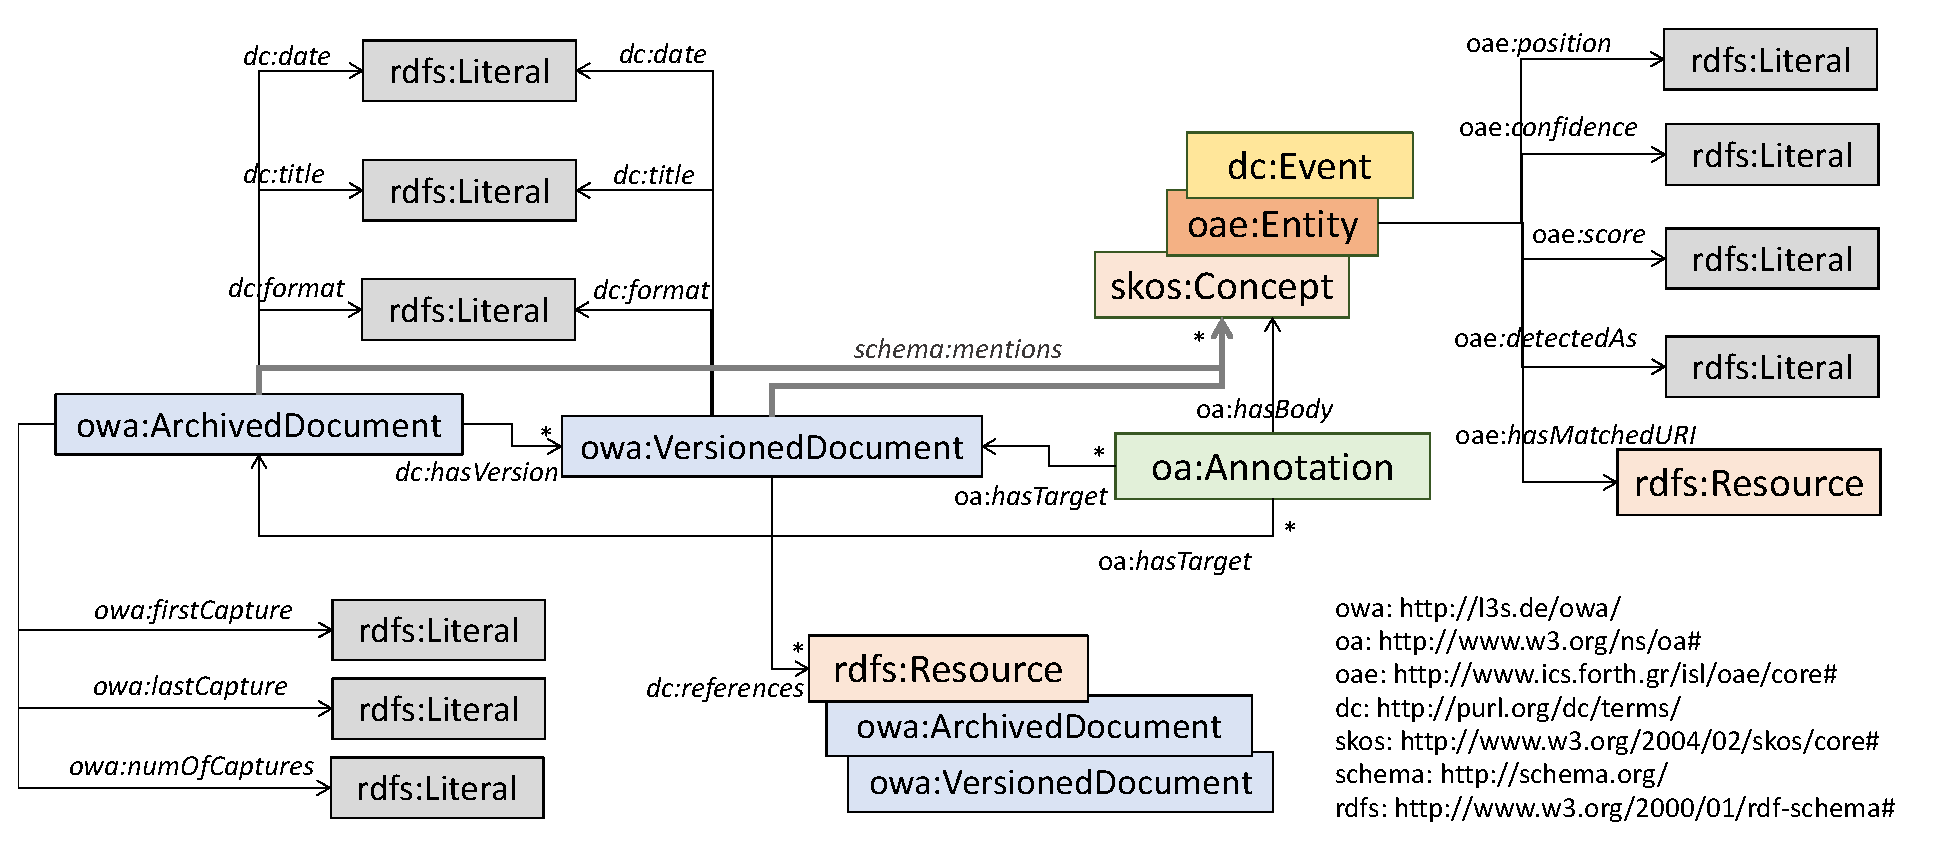
\includegraphics[width=1.0\linewidth]{images/owa.eps}}}\\[0em]%
  \centering{The \emph{Open Web Archive} data model}\\[0.7em]%
  \centering{{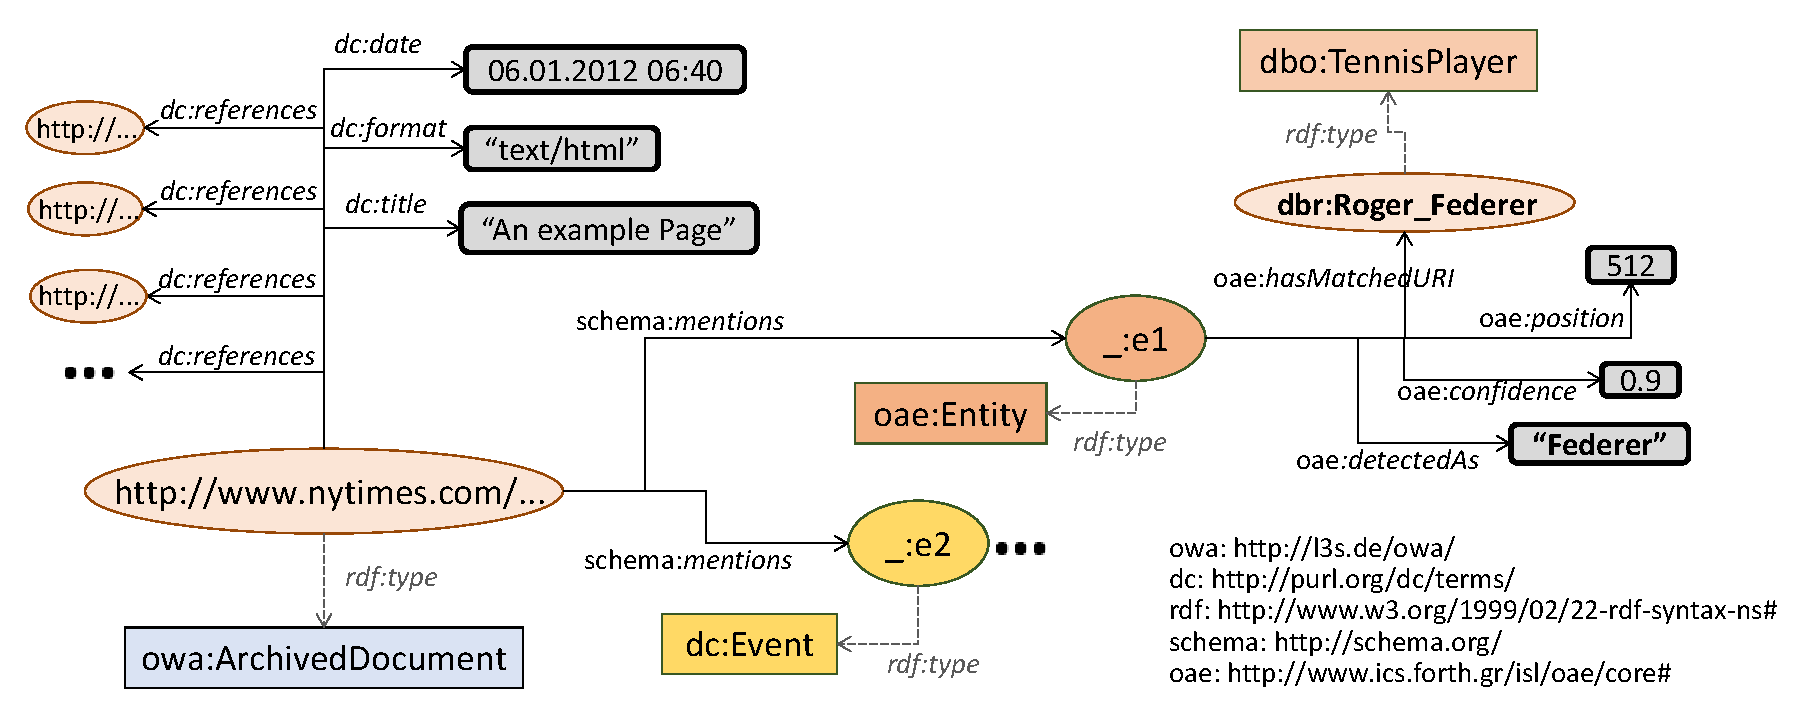
\includegraphics[width=1.0\linewidth]{images/owa_inst_nonvers}}}\\[0em]%
  \centering{Describing an archived article (non-versioned) using the \emph{Open Web Archive} data model}\\[0.7em]%
  \centering{{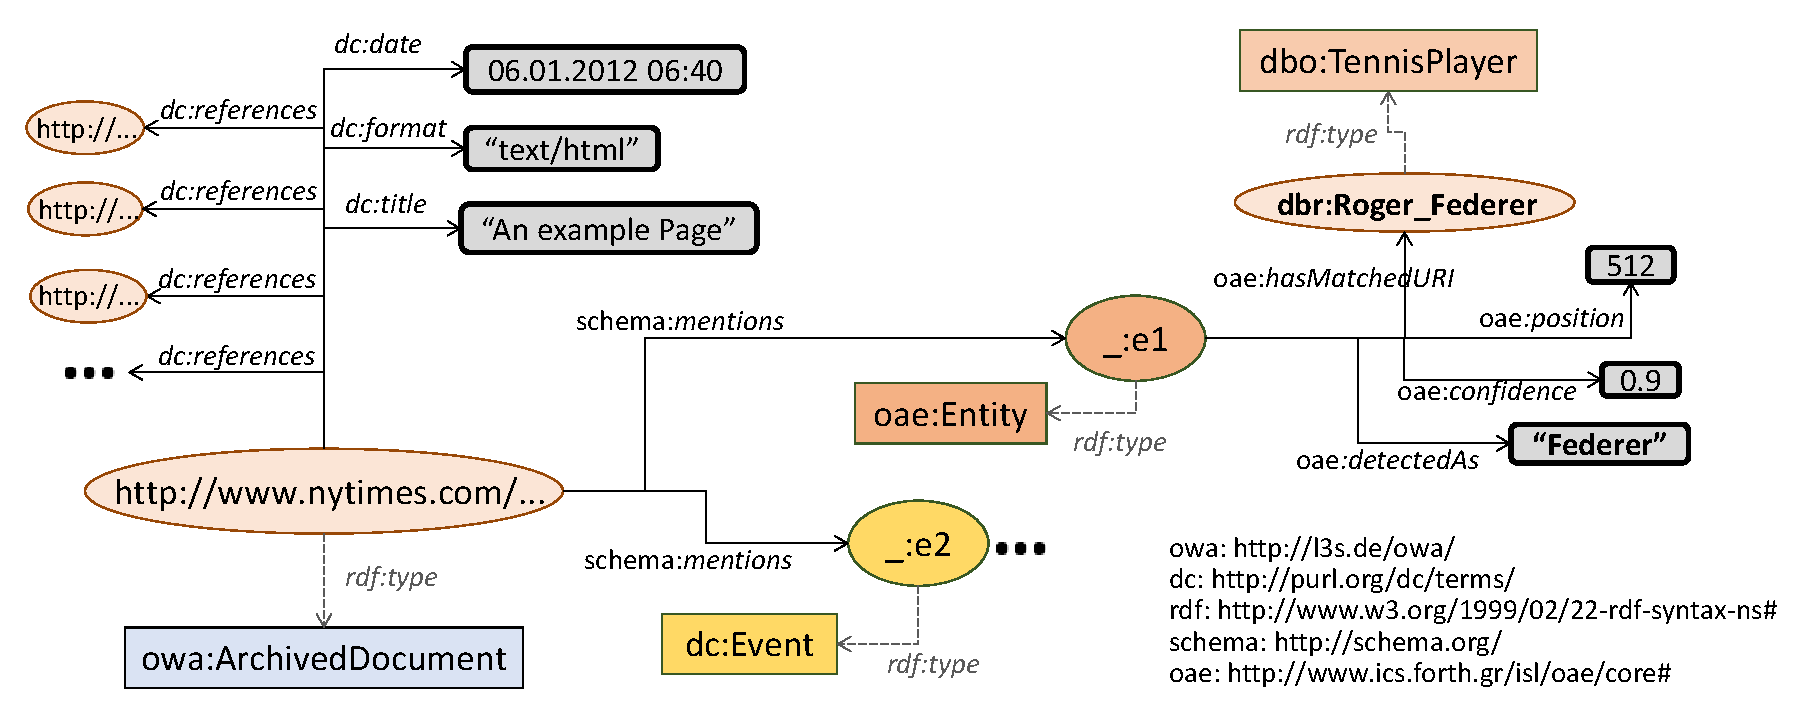
\includegraphics[width=1.0\linewidth]{images/owa_inst_nonvers}}}\\[0em]%
  \centering{Describing an archived web page (versioned) using the \emph{Open Web Archive} data model}\\[0em]%
  \vspace{0.3em}
}
%%%%%%%%%%%%%%%%%%%%%%%%%%%%%%%%%%%%%%%%%%%%%%%%%%%%%%%%%%%%%%%%%%%%%%%%%%%%%%
  \headerbox{Framework}{name=framework,column=1,span=2, below=model}{
%%%%%%%%%%%%%%%%%%%%%%%%%%%%%%%%%%%%%%%%%%%%%%%%%%%%%%%%%%%%%%%%%%%%%%%%%%%%%%
   \smaller%
   \centering{{\includegraphics[width=0.9\linewidth]{images/semlayer_framework.eps}}}\\[0.7em]%
   \centering{The process of construction and querying of Semantic Layers}\\[0em]%
   \vspace{0.3em}
  }
%%%%%%%%%%%%%%%%%%%%%%%%%%%%%%%%%%%%%%%%%%%%%%%%%%%%%%%%%%%%%%%%%%%%%%%%%%%%%%  
  \headerbox{Source Code}{name=source,column=2,below=framework,above=bottom}{
%%%%%%%%%%%%%%%%%%%%%%%%%%%%%%%%%%%%%%%%%%%%%%%%%%%%%%%%%%%%%%%%%%%%%%%%%%%%%%
  \noindent
  \begin{minipage}{\linewidth}
  \begin{minipage}{0.75\linewidth}
    \indent{}The Semantic Layers are publicly available at: 
    \url{http://l3s.de/owa/semanticlayers/}
  \end{minipage}\hfill%
  \begin{minipage}{0.23\linewidth}
  \hfill\includegraphics[width=\linewidth]{semlayer_code}
  \end{minipage}
  \end{minipage}
  \vspace{1em}
  \begin{minipage}{\linewidth} 
  \begin{minipage}{0.75\linewidth}
    \indent{}The dataset used for evaluation is available at:  
    \url{http://l3s.de/owa/semanticlayers/SemLayerEval.zip}
  \end{minipage}\hfill%
  \begin{minipage}{0.23\linewidth}
  \hfill\includegraphics[width=\linewidth]{eval_code}
  \end{minipage}  
  \end{minipage}
  }
%%%%%%%%%%%%%%%%%%%%%%%%%%%%%%%%%%%%%%%%%%%%%%%%%%%%%%%%%%%%%%%%%%%%%%%%%%%%%%
  \headerbox{Future Work}{name=questions,column=1,span=1,below=framework,above=bottom}{
%%%%%%%%%%%%%%%%%%%%%%%%%%%%%%%%%%%%%%%%%%%%%%%%%%%%%%%%%%%%%%%%%%%%%%%%%%%%%%
   \begin{enumerate}\compresslist
   \item Regarding future work and research,
         user-friendly interfaces should be
         developed on top of semantic layers for allowing
         end-users to easily and efficiently explore web archives.
   \item Another interesting direction is to study approaches
         for ranking the results returned by SPARQL queries.
   
   \end{enumerate}
   \vspace{0.3em}
  }
%%%%%%%%%%%%%%%%%%%%%%%%%%%%%%%%%%%%%%%%%%%%%%%%%%%%%%%%%%%%%%%%%%%%%%%%%%%%%%
  \headerbox{Results}{name=res,column=0,below=contribution,above=bottom}{
%%%%%%%%%%%%%%%%%%%%%%%%%%%%%%%%%%%%%%%%%%%%%%%%%%%%%%%%%%%%%%%%%%%%%%%%%%%%%%
  We have introduced a model and a framework
  for describing and publishing metadata and
  semantic information about web archives.
  The constructed {\em semantic layers} allow:
  \begin{enumerate}\compresslist
  \item exploring web archives in a more advanced way
  based on entities, events and concepts extracted
  from the archived documents and linked with web resources.
  \item integrating information coming from multiple knowledge bases 
  and semantic layers.
  \item inferring new knowledge that is very laborious to derive 
  otherwise.
  \item coping with common problems when exploring web archives like
  temporal reference variants and multilinguality.
  \item making the contents of web archives machine understandable,
  thereby enabling their direct exploitation by other systems and
  tools.
  \end{enumerate}
  The results showed that semantic layers
  can answer complex information needs that keyword-based search systems
  fail to satisfy.  
  \vspace{0.3em}
  }

\end{poster}

\end{document}